\documentclass[10pt,a4paper,twocolumn]{article}
\RequirePackage[italian]{babel}
\usepackage{lipsum}
\usepackage{pgfplots}
\usepackage[utf8]{inputenc}
\usepackage{amsmath}
\usepackage{amsfonts}
\usepackage{amssymb}
\usepackage{graphicx}
\usepackage[plainpages=false]{hyperref}
%\usepackage[all]{hypcap} 
\usepackage{fancyhdr}
\usepackage{sectsty}
\usepackage[a4paper, total={6.5in, 9in}]{geometry}
%\DeclareMathSizes{10pt}{13pt}{13pt}{13pt}



\sectionfont{\fontsize{13}{7}\selectfont}
\subsectionfont{\fontsize{11}{12}\selectfont}


\author{Marco Faretra, Gabriele Marini}
\title{\textbf{Big Data Analysis on NBA \& NCAA}\\Colleges' impact on professionistic games}
\begin{document}
	
\maketitle
\thispagestyle{empty}
\pagestyle{empty}
		
\section*{RIASSUNTO}

Lo scopo di questo progetto è quello di produrre un ranking dei college americani sulla base delle performance dei primi anni di carriera dei giocatori professionisti. Allo scopo si sono analizzate tutte le statistiche dei giocatori NBA dai primi anni '50 fino ad oggi e si è semplificato il gioco fino ad individuare 7 categorie di giocatori, non mutuamente esclusive.
Ad ogni giocatore viene assegnato un punteggio a seconda della particolare categoria che si sta analizzando, il punteggio di un college è la somma di tutti i punteggi dei giocatori provenienti da quel college, tenendo conto della particolare categoria analizzata. Lo scopo dell'analisi è quello di comprendere come alcuni college possano puntare su particolari aspetti del gioco, scelta che si dovrebbe riflettere nelle statistiche dei primi anni di carriera di un giocatore professionistico. Inoltre è interessante comprendere come alcuni college possano o meno essere emersi durante lo scorrere del tempo, oppure se le gerarchie tra questi siano rimaste immutate nel passare degli anni. Un'ulteriore analisi riguarda l'aggregazione dei dati ottenuti dal ranking ad un livello di granularità più grande possibile, ovvero al livello degli stati. Questa analisi ulteriore potrebbe portare a comprendere come alcuni stati siano favoriti rispetto ad altri nello sviluppo delle caratteristiche dei giocatori, o del gioco in generale, a seconda di numerosi aspetti come ad esempio il clima la cultura dello stato.

\section{INTRODUZIONE} 

La lega di pallacanestro professionistica americana, meglio conosciuta come NBA, è stata una delle prime realtà a fruire dei dati dei suoi giocatori allo scopo di perfezionare questi ultimi e rendere le franchigie partecipanti sempre più competitive. Questo flusso di dati permette oggigiorno di avere a disposizione una quantità di dati immensa, delle tipologie più disparate, dalle statistiche dei singoli giocatori o delle singole partite, fino ad arrivare alle statistiche più dettagliate play-by-play \footnote{https://www.bigdataball.com/nba-historical-playbyplay-dataset}.

Quello che non tutti sanno è che esiste un mondo dietro a quello della lega professionistica, altrettanto vasto, ovvero quello dei college e della NCAA. Prima di rendersi disponibili per il draft \footnote{Evento in cui 60 giocatori provenienti da tutto il mondo vengono scelti per integrarsi nelle franchigie partecipanti al campionato} i giocatori tendono a svolgere qualche anno di preparazione in uno dei molti college americani. Questi, oltre che a fornire borse di studio ai giocatori, permettono loro di affinare gli aspetti legati al gioco, oltre che a dare loro una discreta visibilità agli occhi degli scout NBA. Le regole per essere eleggibili ad un draft e quindi sperare di entrare nella NBA sono cambiate di molto negli ultimi anni, infatti attualmente vige un limite di età di 19 anni ed una necessità di frequentazione di un college pari a due anni prima di potersi rendere eleggibile. Queste modifiche del regolamento si riflettono nei dati, in quanto in passato era molto più frequente non passare per lo step del college e rendersi eleggibili direttamente finita la high scool, procedimento come già detto non più possibile. Dunque nell'analisi si vedrò un numero di giocatori provenienti dai college molto più alto se si analizzano gli ultimi 20-25 anni, rispetto a se si analizzasse il periodo dagli anni '50 agli anni '80.

Per questo progetto è di interesse la correlazione tra gli insegnamenti del college e l'effettiva applicazione di questi nella sfera professionistica. Il nostro scopo è quello di analizzare, utilizzando tecniche Big Data, le statistiche di tutti i giocatori NBA dai primi anni '50 fino ad oggi, al fine di stilare una classifica dei college americani che hanno avuto nella loro storia almeno un giocatore che è riuscito a fare il salto di categoria nella lega professionistica. Oltre a questo tipo di analisi, fissata come punto di partenza, si è anche voluto espandere l'analisi a due differenti granularità: una più fine, riguardante i giocatori, stilando un ranking dei giocatori per ogni categoria; una più grossolana riguardante gli stati, stilando un ranking degli stati sulla base dei college che risiedono sul territorio dello stato, sommando i risultati di questi college. 

A tale scopo si sono individuate 7 categorie di giocatori: tiratori (divisa a sua volta in tiratori da 2 e tiratori da 3), rimbalzisti, all-around, +/- guys, difensori, attaccanti. Per ognuna di queste categorie si è calcolato una score per ogni giocatore sulla base di alcune particolari statistiche tra le molte disponibili\footnote{per i tiratori, ad esempio, è di fondamentale importanza la \% del tiro, mentre le statistiche relative ai rimbalzi sono state ignorate}. Ogni giocatore contribuisce, per la particolare categoria scelta, al punteggio totale del college di appartenenza, ed ogni college allo stato di appartenenza. In questo modo college che curano di più una particolare caratteristica avranno un punteggio più alto se analizziamo la categoria legata a quella caratteristica. Una volta calcolato lo score per ogni categoria e per ogni college è possibile stilare un ranking dei college categoria per categoria.


\section{SETTING}

Non avendo a disposizione un dataset già pronto si sono utilizzati i dati messi a disposizione da BasketBall-Reference, utilizzando delle procedure standard di estrazione dati da web si è ricavato un sottoinsieme dei dati offerti dal dominio, sono stati scartati tutti i dati relativi ai play-off, alle summer-league, prendendo solamente i dati relativi alle regular seaons. Una volta ottenuti i dati, questi sono stati riversati all'interno sia di un document store che all'interno di un key-value store, con le dovute differenze di modellazione.

\section{APPROCCIO}

Una volta estratti i dati, è stato scelto un document store, per salvare tutti i dati estratti. Il document store è stato affiancato ad un key-value store per il salvataggio dei profili storici dei giocatori.

Una volta preparati i due stores, si può iniziare l'elaborazione dei dati vera e propria utilizzando Spark. Il software eseguibile prevede due modalità di esecuzione: locale e distribuita. Per brevità si analizzerà solamente la modalità locale \footnote{La modalità distribuita è molto simile, l'unica differenza è la distribuzione delle dipendenze ai vari worker. Le altre variazioni vengono gestite mediante delle opzioni passate allo script principale.}.

Ad ogni giocatore viene associato uno score, questa operazione viene eseguita per ogni categoria definita. Prima i giocatori vengono filtrati utilizzando delle soglie, queste sono adattive, a seconda dell'andamento della stagione del giocatore correntemente analizzata possono variare ed essere più o meno permissive. 

Le soglie sono state fissate per un semplice motivo, se vediamo le statistiche nude e crude vi sono dei problemi legati ai giocatori poco utilizzati, questi possono essere stati impiegati nel così detto "trash-time", ovvero quando la partita è già conclusa e mancano pochi minuti al termine. Questi giocatori possono aver realizzato un solo tiro su uno solo tentato, avendo di fatto una percentuale di tiro pari al 100\%. Figure di questo genere sono molto più frequenti di quanto si possa pensare, falsando l'analisi poiché questi tendono ad ottenere un punteggio molto alto grazie alle loro statistiche "stellari".

Un altro caso da gestire è la sovrapposizione di statistiche tra due categorie, si prenda ad esempio le due categorie dei tiratori: tiratori da due e tiratori da tre. Per quanto riguarda la prima categoria una delle percentuali fondamentali è la percentuale di tiro, quanto più è alta tanto più un giocatore può essere considerato un tiratore. Uno dei problemi che sorgono però riguarda i centri o pivot, questi tendono a tirare da molto vicino, spesso schiacciando la palla all'interno del canestro, il risultato è quello di avere delle percentuali di tiro molto più alte della media, tuttavia non possono essere categorizzati come tiratori.

Le soglie servono dunque sia ad aggiungere della semantica ai dati estratti, sia a discernere tra giocatori insignificanti al fine dell'analisi e giocatori che invece devono essere inclusi nell'analisi poiché significanti.

Se il giocatore passa il filtraggio allora a seconda della categoria si tengono in considerazione solo alcune statistiche, queste vengono pesate e sommate tra loro in modo tale da ottenere il risultato finale per il giocatore: \[\sum_{stats}^{} player\_stat_{i} * w_{i} \pm b_{i}\] Per alcune categorie si sono definiti anche alcuni bonus/malus per rendere lo score più particolareggiato.

Non vengono analizzate tutte le stagioni di un giocatore ma solamente le prime 4\footnote{Poiché la carriera professionistica di un giocatore dura mediamente 4.8 anni}, questo perché dopo un certo periodo di permanenza nella lega professionistica alcuni giocatori acquisiscono alcune abilità tipiche dalla squadra per cui giocano, di fatto "eliminando" o comunque rendendo non più distinguibile la linea tra abilità collegiali e abilità acquisite successivamente.

Per tenere in conto quanti più giocatori possibili, anche quelli che hanno avuto meno di 4 anni di militanza nella lega, o perché hanno smesso prima, o perché ricadono nella categoria "rookie" (primo anno di carriera) o "sophomore" (due anni di carriera), il punteggio ottenuto da un giocatore è diviso per il numero di anni di permanenza nella lega, quindi da un minimo di 1 ad un massimo di 4.

\section{SOLUZIONE TECNOLOGICA}

\begin{figure}[h]
	\centering
	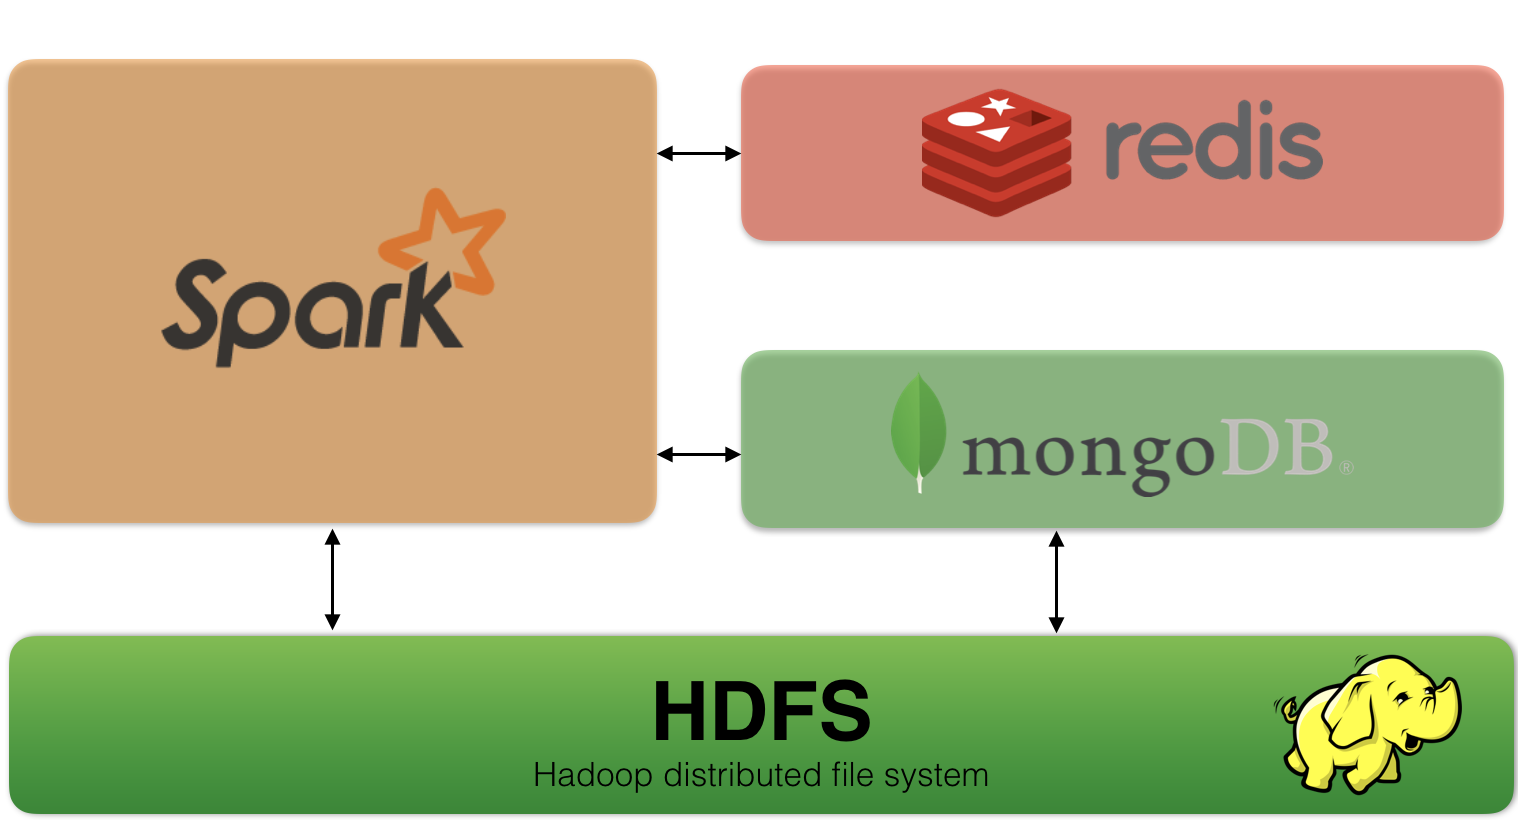
\includegraphics[width=\linewidth]{arch}
	\caption{L'architettura scelta, per la persistenza e per l'elaborazione distribuita}
	\label{fig:arch}
\end{figure}

\begin{figure*}[h]
	\centering
	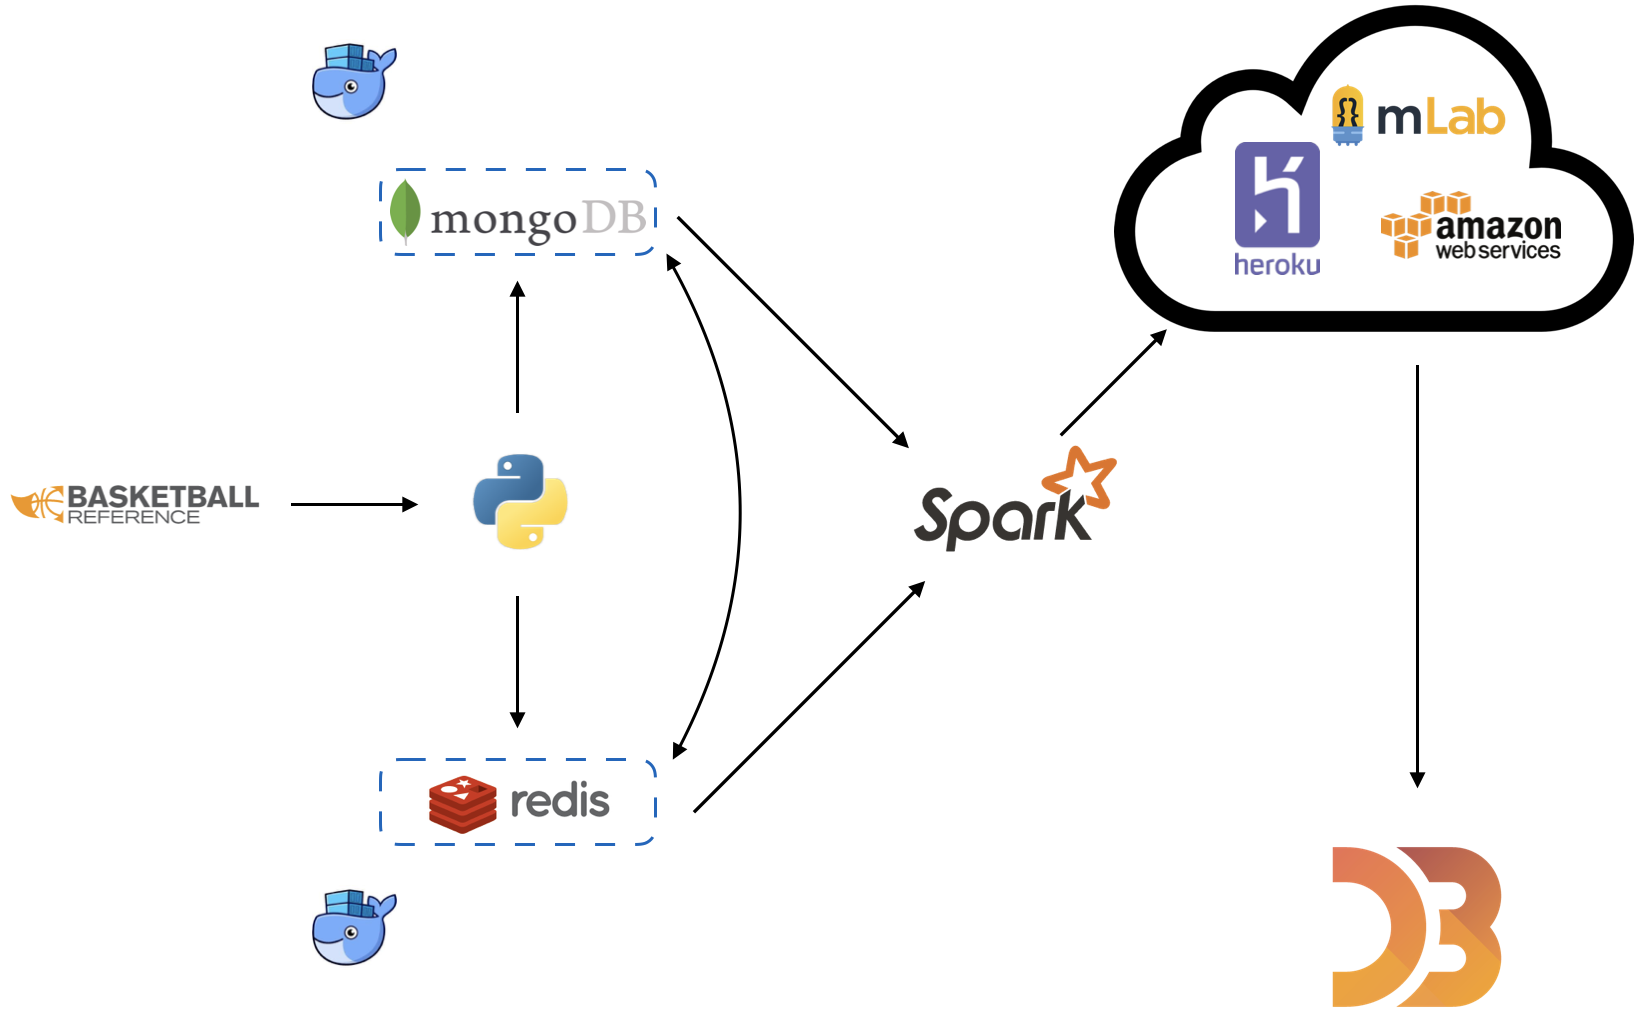
\includegraphics[width=0.8\linewidth]{final}
	\caption{Architettura finale}
	\label{fig:finale}
\end{figure*}

Il linguaggio di riferimento scelto per orchestrare la computazione è Python, grazie alla sua estrema flessibilità e alla possibilità di prototipare una soluzione in breve tempo. Il motore di elaborazione è costituito principalmente da PySpark e Spark MLlib, sono presenti a contorno alcune librerie per il calcolo matematico offerte dall'ecosistema Python come NumPy.

MongoDB è stato scelto per salvare i dati estratti, permette un veloce inserimento dei documenti all'interno del database, soprattutto se questi non hanno necessità di essere messi in relazione, oltre a queste motivazioni, l'ampia diffusione di questo sistema porta con se anche numerose librerie e connettori di supporto.
Inoltre la possibilità di ridurre ancora di più i tempi necessario all'ottenimento di un prototipo è stata forse la motivazione principale per la scelta di questo tipo di tecnologia.
Per quanto riguarda il salvataggio dei dati nel key-value store, il sistema scelto è stato Redis, fondamentalmente a causa della larga diffusione che porta con se documentazione e librerie di supporto. Questo sistema è stato utilizzato per salvare i profili dei giocatori, legando il profilo storico di un giocatore al suo identificatore. A differenza di MongoDB, Redis non è stato affiancato ad un connettore per Spark, infatti uno dei temi che si è voluto affrontare nella sperimentazione, è stato quello della valutazione della bontà dei connettore di MongoDB, eseguendo anche dei test comparativi nella fase di parallelizzazione dei dati, i quali hanno visto MongoDB palese vincitore.

A seguito della preparazione è necessario un ultimo passaggio per completare il setup: con l'aiuto di Spark MLlib si calcolano media, varianza, massimo e minimo per ogni statistica in una particolare stagione; il procedimento viene ripetuto per ogni stagione disponibile. Per alcune statistiche questo procedimento può essere più complicato: alcuni aspetti del gioco sono variati nel corso degli anni, ad esempio dal 1979 è stato introdotto il tiro da 3 punti, giocatori che hanno giocato precedentemente alla stagione 1979-1980 non hanno le statistiche associate al tiro da 3, oppure alcune statistiche non sono rese disponibili prima di una certa stagione. Queste anomalie nei dati costringono a ripensare la gestione delle statistiche, in particolar modo al fine di poter confrontare giocatori moderni con quelli del passato.

Per parallelizzare i dati verso i worker si possono utilizzare entrambi gli stores, tuttavia come già detto MongoDB è fornito di connettore apposito per Hadoop/Spark, mentre redis non utilizza un connettore ma parallelizza i record utilizzando più volte la primitiva "parallelize()" di Spark. Si può definire inoltre l'indirizzo ip della macchina su cui risiedono gli stores, in maniera da cambiare la posizione del server principale secondo bisogno, questa possibilità è utile anche nel caso in cui si voglia lanciare la computazione su un cluster, infatti l'indirizzo del server in cui risiedono i dati non è hard-coded ma passato come parametro ad ogni esecuzione. Sono possibili anche configurazioni diverse in cui i dati sono sparsi su più server, ad esempio si può utilizzare un server per store.

Se si è scelto MongoDB come fornitore dei dati, i worker prendono i dati dal server principale utilizzando il connettore Hadoop-MongoDB, realizzando un RDD che rappresenta una collezione di documenti; se invece si è scelto di utilizzare Redis verranno creati vari RDD e poi uniti a mano a mano fino a formare un singolo RDD. La computazione avviene come descritto in precedenza su ogni singolo RDD.

Alla fine della computazione, se si è scelto di analizzare i giocatori, si ottengono una serie di coppie rappresentanti al primo membro gli identificatori dei giocatori ed al secondo membro lo score associato alla categoria scelta prima di lanciare l'analisi. Se invece si è scelto di analizzare i college si otterranno una serie di triple, in cui il primo membro è il nome del college, il secondo è lo score associato alla particolare categoria scelta, mentre il terzo è il numero di giocatori che hanno frequentato quel college.

All'interno del progetto sono disponibili dei banali strumenti per eseguire alcune aggregazioni di base una volta calcolati tutti gli score. Inoltre è disponibile, in allegato al progetto, una visualizzazione realizzata a partire dai risultati ottenuti al termine delle varie esecuzioni; questa permette di vedere i dati ad un diverso livello di aggregazione: stato $\rightarrow$ college $\rightarrow$ giocatore, oltre alle precedenti aggregazioni è possibile anche esplorare la carriera di un singolo giocatore in forma compatta, analizzando le statistiche per partita di ogni stagione giocata\footnote{https://github.com/gabmarini/infovis\_NBA}.

\section{RISULTATI}

In calce è possibile trovare i risultati dei primi 10 giocatori e dei primi 10 college per ogni categoria.

Di seguito invece i risultati temporali ottenuti facendo partire un'analisi dei college sulla categoria "attaccanti", utilizzando 1 master e 19 nodi (task), da notare che la scala usata è logaritmica sia per apprezzare meglio il punto di incontro tra le due linee, sia per avere una rappresentazione più compatta alla destra del grafico, ovvero laddove si ha un numero elevato di record\footnote{Tutte le categorie hanno una modalità di calcolo molto simile, le differenze temporali non sono apprezzabili cambiando categoria analizzata.}. La macchina utilizzata per i test in locale è la seguente:
\begin{itemize}
	\item MacBook Pro mid 2012
	\item CPU: 2.5GHz Intel Core i5
	\item 12 GB RAM
	\item 500 GB HDD
\end{itemize}

La tipologia di macchine utilizzate per eseguire i test sul cluster è la seguente:
\begin{itemize}
	\item m3.xl
	\item 4vCPU
	\item 15GB RAM
	\item 40GB x 2 SSD
\end{itemize}

\begin{tikzpicture}
\begin{axis}[
width=0.47\textwidth,
xmode=log,
ymode=log,
ymax=50000,
unbounded coords=discard,
grid=both,
grid style={line width=.2pt, draw=gray!10},
major grid style={line width=.3pt,draw=gray!50},
log ticks with fixed point,
title={\texttt{Risultati temporali}},
xlabel=records,
ylabel=secondi,
mark size=2pt,
legend style={at={(0.03,0.85)},anchor=west}
]
\addplot coordinates {
	(100,25)
	(500,56)
	(1000,90)
	(2000,144)
	(4000,265)
	(8000,420)
	(12000,631)
	(30000,1525)
	(45000,2268)
	(60000,3012)
	(75000,3755)
	(90000,4499)
	(105000,5242)
	(120000,5986)	};

\addplot coordinates {
	(100,33)
	(500,46)
	(1000,48)
	(2000,52)
	(4000,56)
	(8000,63)
	(12000,76)
	(30000,128)
	(45000,171)
	(60000,213)
	(75000,256)
	(90000,299)
	(105000,342)
	(120000,385)
	
};

\draw (axis cs:12000,0) -- (axis cs:12000,50000);

\legend{locale, cluster}


\end{axis}
\end{tikzpicture}

I tempi sono stati ottenuti analizzando fino a 12000 giocatori ovvero 407M di statistiche\footnote{Questo limite è rappresentato dalla linea verticale presente nel grafico all'ascissa 12000}, i valori superiori a questa soglia sono stati previsti utilizzando i valori precedentemente ottenuti e una funzione di regressione lineare. Già dall'analisi di poche centinaia di record il tempo di esecuzione del cluster risulta inferire al tempo di esecuzione in locale.

Oltre ai tempi precedenti si sono anche presi i tempi in locale con una macchina più prestante, per testare ulteriormente la bontà degli algoritmi in gioco: 
\begin{itemize}
	\item MacBook Pro 2017
	\item CPU: 2.9GHz Intel Core i7
	\item 16 GB RAM
	\item 500GB SSD
\end{itemize}

I risultati ottenuti sono i seguenti, valgono tutte le considerazioni già fatte per quanto riguarda il metodo di misurazione e i record usati per la misurazione:

\begin{tikzpicture}
\begin{axis}[
width=0.47\textwidth,
xmode=log,
ymode=log,
ymax=50000,
unbounded coords=discard,
grid=both,
grid style={line width=.2pt, draw=gray!10},
major grid style={line width=.3pt,draw=gray!50},
log ticks with fixed point,
title={\texttt{Risultati temporali}},
xlabel=records,
ylabel=secondi,
mark size=2pt,
legend style={at={(0.03,0.85)},anchor=west}
]
\addplot[green, mark=*] coordinates {
	(100,13)
	(500,28)
	(1000,42)
	(2000,65)
	(4000,111)
	(8000,187)
	(12000,278)
	(30000,668)
	(45000,992)
	(60000,1317)
	(75000,1642)
	(90000,1966)
	(105000,2291)
	(120000,2616)	};

\addplot coordinates {
	(100,33)
	(500,46)
	(1000,48)
	(2000,52)
	(4000,56)
	(8000,63)
	(12000,76)
	(30000,128)
	(45000,171)
	(60000,213)
	(75000,256)
	(90000,299)
	(105000,342)
	(120000,385)
	
};

\draw (axis cs:12000,0) -- (axis cs:12000,50000);

\legend{locale, cluster}


\end{axis}
\end{tikzpicture}

Interessante vedere come il punto di incrocio tra le due linee si sposti verso destra arrivando al punto di ascissa 1050 circa, inoltre è possibile vedere come la forbice tra i tempi di elaborazione del cluster e quelli locali si chiuda molto di più rispetto ai tempi presi con la precedente macchina.

L'unica categoria che differisce per quanto riguarda le misurazioni temporali è quella dei "+/- guys", questa è di poco più complicata rispetto alle altre, ovvero include uno spettro di statistiche più ampio rispetto alle altre categorie. Di seguito i tempi presi con la prima macchina di cui si sono viste le specifiche:

\begin{tikzpicture}
\begin{axis}[
width=0.47\textwidth,
xmode=log,
ymode=log,
ymax=50000,
unbounded coords=discard,
grid=both,
grid style={line width=.2pt, draw=gray!10},
major grid style={line width=.3pt,draw=gray!50},
log ticks with fixed point,
title={\texttt{Risultati temporali}},
xlabel=records,
ylabel=secondi,
mark size=2pt,
legend style={at={(0.03,0.85)},anchor=west}
]
\addplot coordinates {
	(100,33)
	(500,73)
	(1000,117)
	(2000,187)
	(4000,345)
	(8000,546)
	(12000,820)
	(30000,1982)
	(45000,2948)
	(60000,3915)
	(75000,4882)
	(90000,5848)
	(105000,6815)
	(120000,7781)	};

\addplot coordinates {
	(100,38)
	(500,53)
	(1000,57)
	(2000,60)
	(4000,64)
	(8000,72)
	(12000,87)
	(30000,147)
	(45000,196)
	(60000,245)
	(75000,295)
	(90000,344)
	(105000,393)
	(120000,442)
	
};

\draw (axis cs:12000,0) -- (axis cs:12000,50000);

\legend{locale, cluster}


\end{axis}
\end{tikzpicture}

\section{CONCLUSIONI}

Dai risultati possiamo evincere che esistono effettivamente dei college migliori di altri dal punto di vista della qualità dei giocatori che escono da questi ultimi, l'analisi storica eseguita dimostra che i college "migliori", sono stati sempre i più affidabili se si vuole fare il salto di qualità nella sfera professionistica.

Alcuni giocatori riconosciuti attualmente come ottimi giocatori risultano avere una posizione abbastanza bassa in classifica, questo è dovuto molto probabilmente al fatto che alcuni di questi giocatori hanno migliorato le loro caratteristiche di gioco più avanti nella carriera e quindi risultano avere uno score basso se si analizzano solo i primi anni di carriera.

Dal punto di vista degli stati è possibile evincere invece che alcuni stati sono privi di college che abbiano avuto un giocatore che sia riuscito a fare il salto di categoria, approdando nell'NBA. Nonostante ci siano dei giocatori originari di questi stati, ad esempio, Carlos Boozer è un famoso giocatore originario dell'Alaska, ma questo stato registra 0 giocatori fatti uscire dai college presenti sul territorio, Boozer ha scelto Duke come college, uno dei migliori che si possano scegliere.

\begin{table*}[t]
	\parbox{.45\linewidth}{
		\begin{tabular}{lc}
			Giocatore & \textit{Plus Minus Score}  \\
			\hline
			Draymond Green & 100.0\\
			Tayshaun Prince & 98.3\\
			Manu Ginobili & 97.16\\
			Josh Howard & 94.34\\
			Kawhi Leonard & 93.89\\
			Tony Parker & 91.71\\
			Rajon Rondo & 90.33\\
			Dwyane Wade & 88.48\\
			Lance Stephenson & 87.92\\
			Klay Thompson & 86.26\\
			&\\
		\end{tabular}
	}
	\quad
	\hspace{20pt}
	\parbox{.45\linewidth}{
		\begin{tabular}{lc}
			Giocatore & \textit{Rebounds Score}  \\
			\hline
			Wilt Chamberlain & 100.0\\
			Bill Russell & 89.19\\
			Jerry Lucas & 74.47\\
			Wes Unseld & 66.6\\
			Maurice Stokes & 66.28\\
			Elgin Baylor & 65.52\\
			Nate Thurmond & 65.07\\
			Walt Bellamy & 64.3\\
			Elvin Hayes & 62.57\\
			Moses Malone & 60.67\\
			&\\
			
		\end{tabular}
	}
	
	
	\parbox{.45\linewidth}{
		\begin{tabular}{lc}
			Giocatore & \textit{3 point shooters Score}  \\
			\hline
			Jason Kapono & 100.0\\
			Stephen Curry & 98.3\\
			Wally Szczerbiak & 97.92\\
			Mark Price & 97.84\\
			Drazen Petrovic & 96.77\\
			Kyle Korver & 96.24\\
			Kelenna Azubuike & 96.12\\
			Trent Tucker & 95.7\\
			Bobby Simmons & 95.1\\
			Jose Calderon & 95.08\\
			&\\
			
		\end{tabular}
	}
	\quad
	\hspace{19pt}
	\parbox{.45\linewidth}{
		\begin{tabular}{lc}
			Giocatore & \textit{Total Score}  \\
			\hline
			Wilt Chamberlain & 455.33\\
			Karl-Anthony Towns & 444.24\\
			Larry Bird & 439.99\\
			Shawn Marion & 439.79\\
			Bill Walton & 427.93\\
			Moses Malone & 427.66\\
			Charles Barkley & 427.62\\
			Kevin Love & 420.92\\
			LeBron James & 415.09\\
			Kawhi Leonard & 415.07\\
			&\\
			
	\end{tabular}}
	
	\parbox{.45\linewidth}{
		\begin{tabular}{lc}
			Giocatore & \textit{All around Score}  \\
			\hline
			Wilt Chamberlain & 100.0\\
			Bill Russell & 89.58\\
			Jerry Lucas & 77.01\\
			Moses Malone & 71.45\\
			David Robinson & 70.52\\
			Bill Walton & 69.84\\
			Wes Unseld & 68.81\\
			Elgin Baylor & 68.08\\
			Maurice Stokes & 68.08\\
			Walt Bellamy & 66.91\\
			&\\
			
		\end{tabular}
	}
	\quad
	\hspace{19pt}
	\parbox{.45\linewidth}{
		\begin{tabular}{lc}
			Giocatore & \textit{2-point shooters Score}  \\
			\hline
			Charles Barkley & 100.0\\
			John Stockton & 99.76\\
			Karl-Anthony Towns & 98.09\\
			Jose Calderon & 96.38\\
			Kiki Vandeweghe & 95.59\\
			Reggie Miller & 94.7\\
			Cedric Maxwell & 94.67\\
			Arron Afflalo & 94.26\\
			Otto Porter & 94.07\\
			Kawhi Leonard & 93.51\\
			&\\
			
	\end{tabular}}
	
	\parbox{.45\linewidth}{
		\begin{tabular}{lc}
			Giocatore & \textit{Attackers Score}  \\
			\hline
			Wilt Chamberlain & 100.0\\
			Elgin Baylor & 74.58\\
			Kareem Abdul-Jabbar & 73.49\\
			Michael Jordan & 71.99\\
			Rick Barry & 71.7\\
			Oscar Robertson & 70.81\\
			Bob McAdoo & 66.87\\
			George Gervin & 66.21\\
			Walt Bellamy & 65.2\\
			Elvin Hayes & 64.25\\
			&\\
			
		\end{tabular}
	}
	\quad
	\hspace{19pt}
	\parbox{.45\linewidth}{
		\begin{tabular}{lc}
			Giocatore & \textit{Defenders Score}  \\
			\hline
			Bill Walton & 100.0\\
			Moses Malone & 74.84\\
			David Robinson & 71.91\\
			Larry Bird & 69.71\\
			Artis Gilmore & 69.35\\
			Tim Duncan & 67.11\\
			Shawn Marion & 64.31\\
			Kevin Love & 64.15\\
			John Shumate & 63.96\\
			Larry Kenon & 63.74\\
			&\\
			
	\end{tabular}}
	
\end{table*}


\begin{table*}[t]
	\begin{tabular}{lc}
		College & \textit{Plus Minus Score}  \\
		\hline
		Marquette University & 100.0\\
		Wake Forest University & 99.97\\
		San Diego State University & 96.85\\
		University of Illinois at Urbana-Champaign & 96.41\\
		University of Oklahoma & 94.84\\
		Washington State University & 94.17\\
		Virginia Commonwealth University & 93.82\\
		Augsburg College & 92.27\\
		Louisiana Tech University & 92.17\\
		University of California & 91.66\\
		&\\
	\end{tabular}
	
	\begin{tabular}{lc}
		College & \textit{Rebounds Score}  \\
		\hline
		University of California, Los Angeles & 100.0\\
		University of Kentucky & 96.67\\
		University of North Carolina & 77.4\\
		Duke University & 68.72\\
		University of Kansas & 66.13\\
		Ohio State University & 54.33\\
		Indiana University & 50.6\\
		University of Louisville & 50.35\\
		University of Michigan & 46.79\\
		University of Arizona & 45.74\\
		&\\
		
	\end{tabular}
	
	\begin{tabular}{lc}
		College & \textit{3 point shooters Score}  \\
		\hline
		University of California, Los Angeles & 100.0\\
		University of North Carolina & 93.1\\
		University of Kentucky & 80.48\\
		University of Arizona & 74.37\\
		Duke University & 70.07\\
		Ohio State University & 57.75\\
		Georgia Institute of Technology & 54.15\\
		Indiana University & 51.82\\
		University of Michigan & 51.63\\
		University of Connecticut & 51.33\\
		&\\
		
	\end{tabular}
	
	\begin{tabular}{lc}
		College & \textit{Defenders Score}  \\
		\hline
		University of California, Los Angeles & 100.0\\
		University of Kentucky & 95.16\\
		University of North Carolina & 85.63\\
		Duke University & 81.23\\
		University of Arizona & 61.42\\
		University of Kansas & 53.6\\
		University of Michigan & 49.1\\
		University of Connecticut & 45.57\\
		Georgetown University & 43.82\\
		Indiana University & 43.27\\
		&\\
		
	\end{tabular}
	
\end{table*}
\begin{table*}[t]
	\begin{tabular}{lc}
		College & \textit{All around Score}  \\
		\hline
		University of California, Los Angeles & 100.0\\
		University of Kentucky & 99.43\\
		University of North Carolina & 81.02\\
		Duke University & 73.44\\
		University of Kansas & 64.36\\
		Indiana University & 52.18\\
		Ohio State University & 51.0\\
		University of Arizona & 50.5\\
		University of Louisville & 49.94\\
		University of Michigan & 48.35\\
		&\\
		
	\end{tabular}
	
	\begin{tabular}{lc}
		College & \textit{2-point shooters Score}  \\
		\hline
		University of California, Los Angeles & 100.0\\
		University of North Carolina & 81.61\\
		University of Kentucky & 70.93\\
		Indiana University & 62.81\\
		Duke University & 53.56\\
		Ohio State University & 51.94\\
		University of Arizona & 51.06\\
		University of Michigan & 46.01\\
		University of Kansas & 42.31\\
		St. John's University & 42.06\\
		&\\
		
	\end{tabular}
	
	\begin{tabular}{lc}
		College & \textit{Attackers Score}  \\
		\hline
		University of Kentucky & 100.0\\
		University of California, Los Angeles & 97.22\\
		University of North Carolina & 95.33\\
		Duke University & 73.22\\
		Indiana University & 60.11\\
		University of Kansas & 58.42\\
		Ohio State University & 54.94\\
		University of Michigan & 50.88\\
		University of Arizona & 46.2\\
		Syracuse University & 45.52\\
		&\\
		
	\end{tabular}
	
	\begin{tabular}{lc}
		College & \textit{Total Score}  \\
		\hline
		University of California, Los Angeles & 663.6\\
		University of North Carolina & 573.92\\
		University of Kentucky & 573.66\\
		Duke University & 420.24\\
		University of Kansas & 392.67\\
		Indiana University & 385.18\\
		University of Arizona & 375.97\\
		Ohio State University & 369.96\\
		University of Michigan & 338.17\\
		University of Notre Dame & 310.25\\
		&\\
		
	\end{tabular}
	
\end{table*}



\end{document}